\documentclass[12pt,a4paper]{article}
\usepackage{hyperref}
\usepackage{graphicx}
\graphicspath{{./images/}}
\hypersetup{
    colorlinks,
    citecolor=black,
    filecolor=black,
    linkcolor=black,
    urlcolor=black
}
\usepackage[T1]{fontenc}
\usepackage[utf8]{inputenc}
\usepackage[polish]{babel}
\usepackage{indentfirst}
\usepackage[margin=0.8in]{geometry}

\usepackage[dvipsnames]{xcolor}

\newcommand{\re}[1]{\textcolor{red}{#1}}

\newcommand{\bl}[1]{\textcolor{blue}{#1}}

\newcommand{\gr}[1]{\textcolor{Plum}{#1}}


\begin{document}
\author{Wojciech Adamiec, 310064}
\title{
	\textbf{Pracownia 0}\\
	\large Analiza Numeryczna (M)
}

\maketitle

\tableofcontents

\section{Tytuł rozdziału numer 1}
Jak co roku obchody lanego poniedziałku w Bełchatowie wywołują wiele emocji. Święto to jest, co prawda, uświęcone tradycją, jednakże są ludzie, którzy zdecydowanie przesadzają z hołdowaniem tej jednej tradycji. „Świństwo, kiedyś to dziewczyny się perfumami lało, a nie tak, jak teraz, wiadrami; tałatajstwo!!!”, oburza się starszy pan, zapytany o opinię na temat nadchodzącego poniedziałku.

\subsection{Tytuł podrozdziału numer 1.1}
W ubiegłym roku śmigus- dyngus okazał się wyjątkowo mokry i wyjątkowo brzemienny w skutkach. W wyniku „niewinnych” igraszek z wodą doszło do wypadku samochodowego, w wyniku którego jedna osoba doznała poważnych obrażeń kręgosłupa. Było to na szczęście jedyne tak tragiczne wydarzenie owego dnia.

\subsection{Tytuł podrozdziału numer 1.2}
Wczoraj o godzinie osiemnastej odbyło się zebranie Stowarzyszenia Bełchatowskich Rodzin, na którym omawiano drażniący problem lanego poniedziałku. Wysunięto także propozycję, aby na ulicę wyszły prewencyjnie liczniejsze niż zwykle patrole policji i straży miejskiej. Rodziny zaapelowały do młodzieży, żeby ta nie przesadzała z wodą.


\section{Tytuł rozdziału numer 2}
Sed ut perspiciatis, unde omnis iste natus error sit voluptatem accusantium doloremque laudantium, totam rem aperiam eaque ipsa, quae ab illo inventore veritatis et quasi architecto beatae vitae dicta sunt, explicabo. Nemo enim ipsam voluptatem, quia voluptas sit, aspernatur aut odit aut fugit, sed quia consequuntur magni dolores eos, qui ratione voluptatem sequi nesciunt, neque porro quisquam est, qui dolorem ipsum, quia dolor sit, amet, consectetur, adipisci velit, sed quia non numquam eius modi tempora incidunt, ut labore et dolore magnam aliquam quaerat voluptatem. Ut enim ad minima veniam, quis nostrum exercitationem ullam corporis suscipit laboriosam, nisi ut aliquid ex ea commodi consequatur? Quis autem vel eum iure reprehenderit, qui in ea voluptate velit esse, quam nihil molestiae consequatur, vel illum, qui dolorem eum fugiat, quo voluptas nulla pariatur?

\subsection{Tytuł podrozdziału numer 2.1}
At vero eos et accusamus et iusto odio dignissimos ducimus, qui blanditiis praesentium voluptatum deleniti atque corrupti, quos dolores et quas molestias excepturi sint, obcaecati cupiditate non provident, similique sunt in culpa, qui officia deserunt mollitia animi, id est laborum et dolorum fuga. Et harum quidem rerum facilis est et expedita distinctio. Nam libero tempore, cum soluta nobis est eligendi optio, cumque nihil impedit, quo minus id, quod maxime placeat, facere possimus, omnis voluptas assumenda est, omnis dolor repellendus. Temporibus autem quibusdam et aut officiis debitis aut rerum necessitatibus saepe eveniet, ut et voluptates repudiandae sint et molestiae non recusandae. Itaque earum rerum hic tenetur a sapiente delectus, ut aut reiciendis voluptatibus maiores alias consequatur aut perferendis doloribus asperiores repellat.

\subsection{Tytuł podrozdziału numer 2.2}
„Nie ma zatem takiego człowieka, który kocha cierpienie samo w sobie, kto by do niego dążył lub chciał go doświadczyć tylko dlatego, że jest to cierpienie, a dlatego, że czasami zdarzają się takie okoliczności, w których to cierpienie może doprowadzić go do jakiejś wielkiej przyjemności. Dając przykład banalny: któż z nas kiedyś nie podejmował się trudnego wysiłku fizycznego, mając na względzie uzyskanie z tego korzyści? Kto ma jakiekolwiek prawo obwiniać człowieka, który wybiera przyjemność nie wiążącą się z przykrymi konsekwencjami, albo tego, kto unika takiego cierpienia, które nie prowadzi do przyjemności?” (Dalej: „jednocześnie potępiamy ze słusznym oburzeniem i czujemy niechęć do ludzi, którzy są tak owładnięci urokami nietrwałej przyjemności, tak zaślepieni jej pragnieniem, że nie dostrzegają, iż następstwem ich postępowania będą z pewnością cierpienie i trudności.”)

\section{Tytuł rozdziału numer 3}
W imię Boga, w Trójcy Świętej jedynego. Stanisław August [1] z Bożej łaski i woli Narodu Król Polski, Wielki
Książę Litewski, Ruski, Pruski, Mazowiecki, Żmudzki, Kijowski, Wołyński, Podolski, Podlaski, Inflancki,
Smoleński, Siewierski i Czernichowski, wraz ze Stanami Skonfederowanymi, w liczbie podwójnej naród polski
reprezentującymi.
Uznając, iż los nas wszystkich od ugruntowania i wydoskonalenia konstytucji narodowej jedynie zawisł, długim
doświadczeniem poznawszy zadawnione rządu naszego wady, a chcąc korzystać z pory, w jakiej się Europa
znajduje i z tej dogorywającej chwili, która nas samym sobie wróciła, wolni od hańbiących obcej przemocy
nakazów, ceniąc drożej nad życie, nad szczęśliwość osobistą, egzystencję polityczną, niepodległość zewnętrzną i
wolność wewnętrzną narodu, którego los w ręce nasze jest powierzony, chcąc oraz na błogosławieństwo, na
wdzięczność współczesnych i przyszłych pokoleń zasłużyć, mimo przeszkód, które w nas namiętności
sprawować mogą dla dobra powszechnego, dla ugruntowania wolności, dla ocalenia Ojczyzny naszej i jej granic
z największą stałością ducha, niniejszą konstytucję uchwalamy i i; tę całkowicie za świętą, za niewzruszoną
deklarujemy, dopóki by naród w czasie prawem przepisanym, wyraźną wolą swoją nie uznał potrzeby
odmienienia w niej jakiego artykułu.
Do której to konstytucji dalsze ustawy sejmu teraźniejszego we wszystkim stosować się mają. 

\subsection{Tytuł podrozdziału numer 3.1}
Religią narodową panujacą jest i będzie wiara święta rzymska katolicka ze wszystkimi jej prawami; przejście od
wiary panującej do jakiegokolwiek wyznania jest zabronione pod karami apostazji. Że zaś taż sama wiara święta
przykazuje nam kochać bliźnich naszych, przeto wszystkim ludziom jakiegokolwiek bądź wyznania, pokój w
wierze i opiekę rządową winniśmy i dlatego wszelkich obrządków i religii wolność w krajach polskich, podług
ustaw krajowych warujemy. 


\subsection{Tytuł podrozdziału numer 3.2}
Prawo na teraźniejszym Sejmie zapadłe pod tytułem: Miasta Nasze Królewskie wolne w państwach
Rzeczypospolitej [13] w zupełności utrzymane mieć chcemy i za część niniejszej konstytucji deklarujemy, jako
prawo wolnej szlachcie polskiej, dla bezpieczeństwa ich swobód i całości wspólnej Ojczyzny nową, prawdziwą i
skuteczną dające siłę.

\section{Tabele}

\begin{center}
	\begin{tabular}{|l||cr|}\hline
	Imię i Nazwisko & Fajność & Punkty \\ \hline
	A. Jan Kowalski & 3/10 	  & 73 \\
	B. Jan Nowak & 7/10 	  & 273 \\
	C. Adam Wojak & 6/10 	  & 913 \\ \hline
	\end{tabular}
\end{center}

Uwaga! Tabela zawiera całkowicie przypadkowe dane.

\begin{center}
	\begin{tabular}{||c|c|c|c||} \hline
	\multicolumn{4}{||c||}{Funkcja $f(x) = \sin x$} \\ \hline
	Liczba & Metoda 1 & Metoda 2 & Metoda 3 \\ \hline
	10 	   & 0.72     & 0.25     & 0.71     \\
	20 	   & 0.73     & 0.22     & 0.41     \\
	30 	   & 0.52     & 0.02     & 0.33     \\
	40 	   & 0.64     & 0.12     & 0.24     \\
	50 	   & 0.24     & 0.06     & 0.12     \\ \hline
	\end{tabular}
\end{center}

\section{Wykres}
Tutaj mamy wykres losowo wygenerowany przez załączony program.

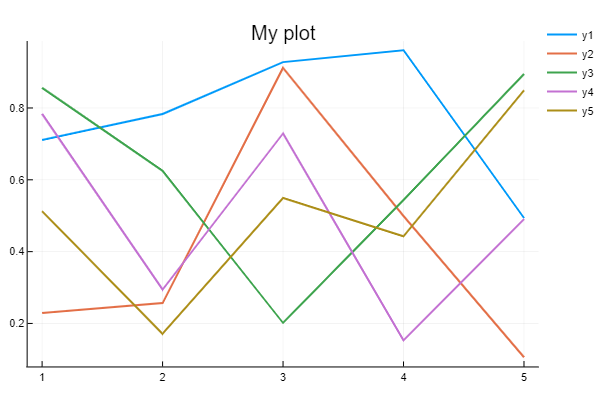
\includegraphics[scale=0.7]{plot}

\section{Twierdzenie Taylora(o szeregu)}

Niech $Y$ będzie przestrzenią unormowaną oraz $f:[a, b] \rightarrow Y$ będzie funkcją $(n + 1)$ razy różniczkowalną na przedziale $[a, b]$ w sposób ciągły (na końcach przedziału zakłada się różniczkowalność z lewej, bądź odpowiednio, z prawej strony). Wówczas dla każdego punktu $x$ z przedziału $(a, b)$ spełniony jest wzór zwany \textit{wzorem Taylora}.

$$f(x) = f(a) + \frac{x-a}{1!}f^{(1)}(a) + ... + \frac{(x-a)^n}{n!}f^{(n)}(a) + R_n(x, a) = \sum_{k=0}^{n} {\frac{(x - a)^k}{k!}f^{k}(a)} + R_n(x, a)$$

Gdzie $f^{(k)}(a)$ jest pochodną k-tego rzędu funkcji $f$, obliczoną w punkcie $a$. $R_n(x, a)$ spełnia warunek:

$$\lim_{x\to a}{\frac{R_n(x, a)}{(x-a)^n}} = 0$$

Funkcja $R_n(x, a)$ nazywana jest resztą Peana we wzorze Taylora. W przypadku $a = 0$, wzór Taylora nazywany jest wzorem Maclaurina.


\end{document}